%!TEX TS-program = pdflatexmk

% Copyright (c) 2018 - 2022, Martin Scheidt (ISC license)
% Permission to use, copy, modify, and/or distribute this file for any purpose with or without fee is hereby granted, provided that the above copyright notice and this permission notice appear in all copies.

\documentclass[border=2]{standalone}

\usepackage[dev]{tikz-trackschematic}

\begin{document}
  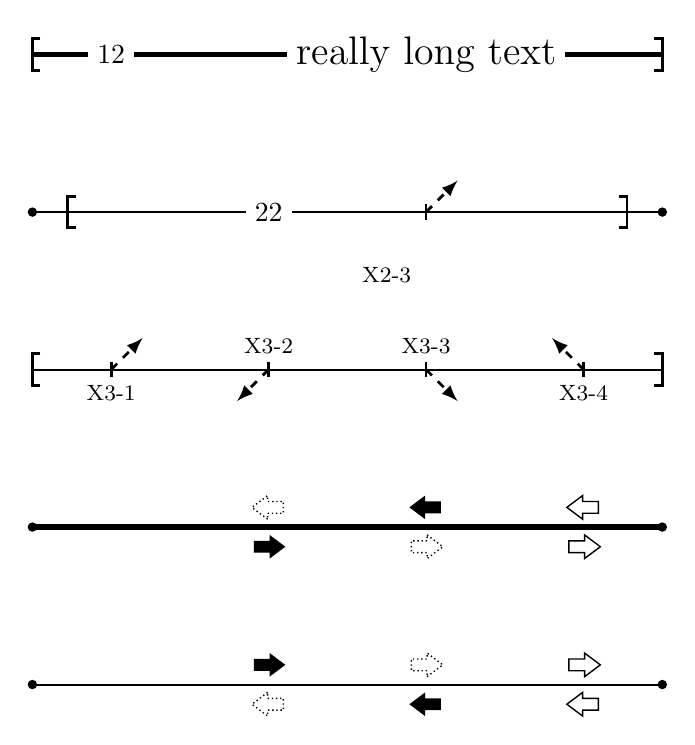
\begin{tikzpicture}
  
    \foreach \i in {1,2,...,5}{% base coordinate
      \coordinate (A\i) at ($(0,0) + 2*(0,-\i)$);% base coordinate
      \coordinate (B\i) at ($(8,0) + 2*(0,-\i)$);% base coordinate
    }

    \foreach \i in {1,4}{% draw main tracks on base coordinate
      \maintrack (A\i) --   (B\i);
    }

    \foreach \i in {2,3,5}{% draw secondary tracks on base coordinate
      \secondarytrack (A\i) --   (B\i);
    }

    \foreach \i in {1,2,...,5}{% coordinates for testing symbols
      \coordinate (X\i-1) at ($(1,0) + 2*(0,-\i)$);
      \coordinate (X\i-2) at ($(3,0) + 2*(0,-\i)$);
      \coordinate (X\i-3) at ($(5,0) + 2*(0,-\i)$);
      \coordinate (X\i-4) at ($(7,0) + 2*(0,-\i)$);
    }

    \tracklabel at (X1-1) label (12);
    \tracklabel at (X1-3) label (\Large really long text);
    \tracklabel at (X2-2) label (22);
    \derailer[forward,branch=left,shift label={(-0.5,-0.5)}] at (X2-3) label (X2-3);

    \derailer[forward ,branch=left ] at (X3-1) label (X3-1);
    \derailer[backward,branch=left ] at (X3-2) label (X3-2);
    \derailer[forward ,branch=right] at (X3-3) label (X3-3);
    \derailer[backward,branch=right] at (X3-4) label (X3-4);

    \bufferstop[backward] at (A1);
    \bufferstop[forward]  at (B1);
    \bufferstop[backward,friction=.5]  at (A2);
    \bufferstop[forward ,friction=.5]  at (B2);
    \bufferstop[backward] at (A3);
    \bufferstop[forward]  at (B3);

    \trackclosure at (A4);
    \directioncontrol[forward] at (X4-2);
    \directioncontrol[backward] at (X4-3);
    \directioncontrol[bidirectional] at (X4-4);
    \trackclosure at (B4);

    \trackclosure at (A5);
    \directioncontrol[forward,position=left] at (X5-2);
    \directioncontrol[backward,position=left] at (X5-3);
    \directioncontrol[bidirectional,position=left] at (X5-4);
    \trackclosure at (B5);

  \end{tikzpicture}
\end{document}